\only<beamer>{\titleframe}

\begin{frame}{Gliederung}
  \tableofcontents[hideallsubsections]
\end{frame}


\section{Einleitung}
\begin{frame}{\insertsection}
  \textit{Selection(n,i):} Finde das $i$ kleinste Element in einer Liste mit $n$ Elementen.

  \vspace{5mm}
  Grundlegende Arbeiten:

  \vspace{2mm}
  \begin{tabular}{|p{6cm}|p{6cm}|}
    \hline
    \multicolumn{1}{|c|}{Gasarch, Kelly and Puth (1996)}                                                                  & \multicolumn{1}{c|}{Oksanen (2002)} \\
    \cline{1-2}
    \raggedright \begin{itemize}
                   \item [...]haben als erste Computersuche angewandt, um untere Schranken für das \textit{Selection}-Problem zu finden.
                   \item [...]nutzten für größere $n,i$ sog. \textit{pair-forming algorithms}
                 \end{itemize} &
    \begin{itemize}
      \item[...] stellte einen Computersuch-Algorithmus online, der die unteren Schranken von Gasarch et al. übertraf.
    \end{itemize}                                             \\
    \cline{1-2}
  \end{tabular}
\end{frame}

\begin{frame}{\insertsection}
  \textbf{Aufgabenstellung} \\
  \vspace{5mm}
  Bestimme mit Computersuche $V_i^n$ - die Anzahl an Vergleichen, die ein optimaler Algorithmus im Worst Case benötigt, um das $i$ kleinste von $n$ Elementen zu finden.

\end{frame}


\section{Grundlagen}

\subsection{Partial Order Sets}

\sectionframe{\insertsection}

\begin{frame}{Zentrale Datenstruktur: Poset}
  \textbf{Definition:}
  \vspace{1mm}
  \begin{itemize}
    \item Sei $\Omega$ eine Menge mit paarweise verschiedenen Elementen mit $\vert \Omega \vert = n$.
    \item $(n,i,R)$ bezeichnet eine Instanz des \textit{Selection}-Problems.
    \item $R \subseteq \Omega^2$ mit $(a,b) \in R \Leftrightarrow a \leq b$.
  \end{itemize}
  \vspace{2mm}
\end{frame}

\begin{frame}{Zentrale Datenstruktur: Poset}
  \textbf{Dualität:} \\
  \vspace{1mm}
  Das Duale eines Posets $P = (n, i, R)$ ist das Poset $P^{-1} = \left(n, n-1-i, R'\right)$ mit $R' = \{ (u,v) \; \vert \; (v,u) \in R\}$.

  \pause
  \vspace{2mm}
  \textbf{Reduktion:} \\
  \vspace{1mm}
  Ein Poset heißt \textit{reduziert}, wenn es zu jedem Element höchstens $i$ viele kleinere Elemente gibt und höchstens $n-1-i$ viele größere Elemente.
\end{frame}

\begin{frame}{Zentrale Datenstruktur: Poset}
  \textbf{Kanonische Form:} \\
  \vspace{1mm}
  Ein Poset heißt \textit{kanonifiziert}, wenn alle Elemente des Posets kanonisch angeordnet sind. Das heißt, dass alle möglichen Permutationen der Elemente auf das Poset abbilden.

  \pause
  \vspace{2mm}
  \textbf{Normalform:} \\
  \vspace{1mm}
  Ein reduziertes und kanonifiziertes Poset heißt \textit{normalisiert}.

  \pause
  \vspace{2mm}
  \textbf{Optimale Kosten:} \\
  \vspace{1mm}
  \textit{Kosten eines Posets} $V(P)$ mit $P=(n,i,R)$ sind die optimale Anzahl an weiteren Vergleichen, die benötigt werden, um das $i$ kleinste Element zu bestimmen.
\end{frame}

\begin{frame}{Ein Lemma}
  \textbf{Lemma 1:} Für ein Poset $P=(n,i,R)$ gilt $V(P) = V(P^{-1})$.
  \vspace{1mm}

  \textit{Beweis: Die Berechnung von $V(P)$ ergibt gleichzeitig einen Algorithmus, der in einen Entscheidungsbaum übersetzt werden kann. Vertausche alle Kinder, und derselbe Algorithmus führt auf die Lösung von $P^{-1}$.}

\end{frame}

\begin{frame}{Ein Beispiel mit Poset-Reduktion}
  \begin{figure}
    \begin{tikzpicture}[tcancel/.append style={draw=#1, cross out, inner sep=6pt}]
  \draw(-.5, -.5) rectangle (4.5, .5);
  \node[circle,draw=black] (A1) at (0, 0) {};
  \node[circle,draw=black] (A2) at (1, 0) {};
  \node[circle,draw=black] (A3) at (2, 0) {};
  \node[circle,draw=black] (A4) at (3, 0) {};
  \node[circle,draw=black] (A5) at (4, 0) {};

  \draw[dashed] (A1) -- (A2) node {};
  \draw[dashed] (A3) -- (A4) node {};

  \draw(-0.5, -2.6) rectangle (4.5, -0.8);
  \node[circle,draw=black] (B1) at (1.0, 0 - 2.2) {};
  \node[circle,draw=black] (B2) at (1.0, 1 - 2.2) {};
  \node[circle,draw=black] (B3) at (2.0, 0 - 2.2) {};
  \node[circle,draw=black] (B4) at (2.0, 1 - 2.2) {};
  \node[circle,draw=black] (B5) at (4.0, 0.5 - 2.2) {};

  \draw (B1) -- (B2) node {};
  \draw (B3) -- (B4) node {};
  \draw[dashed] (B2) -- (B4) node {};

  \draw(-0.5, -5.5) rectangle (4.5, -2.9);
  \node[circle,draw=black] (C1) at (1, 0 - 5.0) {};
  \node[circle,draw=black] (C2) at (1, 1 - 5.0) {};
  \node[circle,draw=black,tcancel=red] (C3) at (2, 1.5 - 5.0) {};
  \node[circle,draw=black] (C3) at (2, 1.5 - 5.0) {};
  \node[circle,draw=black] (C4) at (2, .5 - 5.0) {};
  \node[circle,draw=black] (C5) at (3, .5 - 5.0) {};

  \draw (C1) -- (C2) node {};
  \draw (C3) -- (C4) node {};
  \draw (C2) -- (C3) node {};
  \draw[dashed] (C4) -- (C5) node {};

  \draw(5.5, -1.3) rectangle (10.5, .5);
  \node[circle,draw=black] (D1) at (6, 0.1 - 1) {};
  \node[circle,draw=black] (D2) at (6, 0.1) {};
  \node[circle,draw=black] (D3) at (7, 0.1 - 1) {};
  \node[circle,draw=black] (D4) at (7, 0.1 ) {};
  \node[circle,draw=black,tcancel=red] (D5) at (10.0, 0.1 -0.5) {};
  \node[circle,draw=black] (D5) at (10.0, 0.1 -0.5) {};

  \draw (D1) -- (D2) node {};
  \draw (D3) -- (D4) node {};
  \draw[dashed] (D2) -- (D4) node {};

  \draw(5.5, -4.1) rectangle (10.5, -1.6);
  \node[circle,draw=black,tcancel=red] (E1) at (8, 1.5 - 3.6) {};
  \node[circle,draw=black] (E1) at (8, 1.5 - 3.6) {};

  \node[circle,draw=black] (E2) at (7, 1 - 3.6) {};
  \node[circle,draw=black,tcancel=red] (E3) at (7, 0 - 3.6) {};
  \node[circle,draw=black] (E3) at (7 , 0 - 3.6) {};

  \node[circle,draw=black] (E4) at (8, 0.5 - 3.6) {};

  \node[circle,draw=black,tcancel=red] (E5) at (9, 0.5 - 3.6) {};
  \node[circle,draw=black] (E5) at (9, 0.5 - 3.6) {};

  \draw (E1) -- (E2) node {};
  \draw (E1) -- (E4) node {};
  \draw (E2) -- (E3) node {};
  \draw[dashed] (E2) -- (E4) node {};

\end{tikzpicture}
  \end{figure}

\end{frame}

\subsection{Kompatible Lösungen}
\begin{frame}{\insertsubsection}
  \centering
  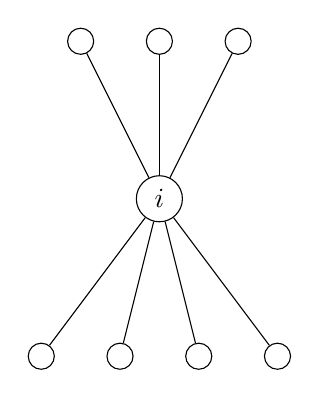
\begin{tikzpicture}

    \node[draw, circle] (l0) at (0, 0) {};
    \node[draw, circle] (l1) at (1, 0) {};
    \node[draw, circle] (l2) at (2, 0) {};
    \node[draw, circle] (l3) at (3, 0) {};

    \node[draw, circle] (I) at (1.5, 2) {$i$};

    \path[draw] (l0) to (I);
    \path[draw] (l1) to (I);
    \path[draw] (l2) to (I);
    \path[draw] (l3) to (I);

    \node[draw, circle] (u0) at (0.5, 4) {};
    \node[draw, circle] (u1) at (1.5, 4) {};
    \node[draw, circle] (u2) at (2.5, 4) {};

    \path[draw] (u0) to (I);
    \path[draw] (u1) to (I);
    \path[draw] (u2) to (I);

  \end{tikzpicture}

\end{frame}

\begin{frame}{\insertsubsection}
  \centering
  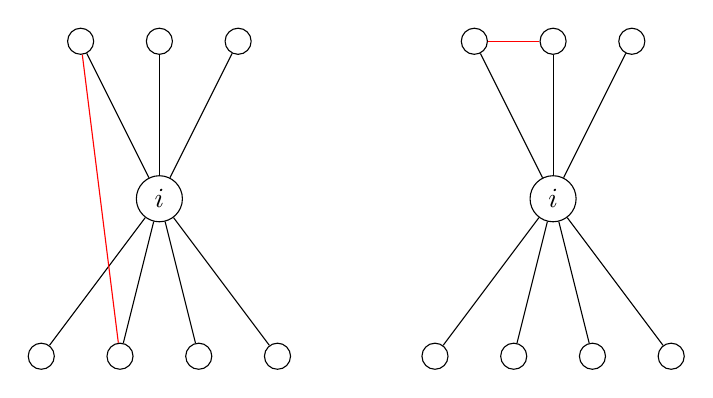
\begin{tikzpicture}

    \node[draw, circle] (fl0) at (0, 0) {};
    \node[draw, circle] (fl1) at (1, 0) {};
    \node[draw, circle] (fl2) at (2, 0) {};
    \node[draw, circle] (fl3) at (3, 0) {};

    \node[draw, circle] (fI) at (1.5, 2) {$i$};

    \path[draw] (fl0) to (fI);
    \path[draw] (fl1) to (fI);
    \path[draw] (fl2) to (fI);
    \path[draw] (fl3) to (fI);

    \node[draw, circle] (fu0) at (0.5, 4) {};
    \node[draw, circle] (fu1) at (1.5, 4) {};
    \node[draw, circle] (fu2) at (2.5, 4) {};

    \path[draw] (fu0) to (fI);
    \path[draw] (fu1) to (fI);
    \path[draw] (fu2) to (fI);

    \path[draw=red] (fu0) to (fl1);

    %second

    \node[draw, circle] (sl0) at (0 + 5, 0) {};
    \node[draw, circle] (sl1) at (1 + 5, 0) {};
    \node[draw, circle] (sl2) at (2 + 5, 0) {};
    \node[draw, circle] (sl3) at (3 + 5, 0) {};

    \node[draw, circle] (sI) at (1.5 + 5, 2) {$i$};

    \path[draw] (sl0) to (sI);
    \path[draw] (sl1) to (sI);
    \path[draw] (sl2) to (sI);
    \path[draw] (sl3) to (sI);

    \node[draw, circle] (su0) at (0.5 + 5, 4) {};
    \node[draw, circle] (su1) at (1.5 + 5, 4) {};
    \node[draw, circle] (su2) at (2.5 + 5, 4) {};

    \path[draw] (su0) to (sI);
    \path[draw] (su1) to (sI);
    \path[draw] (su2) to (sI);

    \path[draw=red] (su0) to (su1);

  \end{tikzpicture}

\end{frame}

\subsection{Kompatible Lösungen}
\begin{frame}{\insertsubsection}
  \centering
  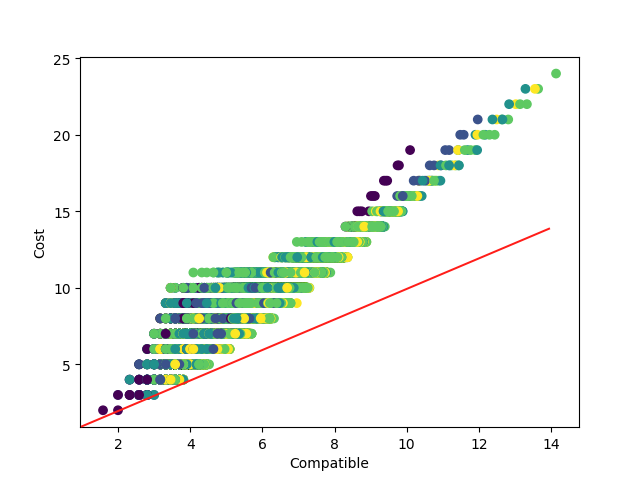
\includegraphics[scale=.5]{../article/figures/compatible_cost_relation.png}

\end{frame}

\section{Vorwärtssuche}
\sectionframe{\insertsection}

\begin{frame}{\insertsection}
  \centering
  \begin{tikzpicture}
    [
      level 1/.style = {sibling distance = 4cm},
      level 2/.style = {sibling distance = 2.5cm},
    ]

    \node[] (root) {$(n,i,\emptyset)$}
    child {
        node[] {$\{a,b\}$}
        child {
            node[] {$(n,i,\{(a,b)\})$}
            child[sibling distance = 1cm] {
                node[] {$\{c,d\}$}
                child[sibling distance = 1cm] { node[] {$\cdots$}}
                child[sibling distance = 1cm] { node[] {$\cdots$}}
              }
            child[sibling distance = 1cm] { node[] {$\cdots$}}
          }
        child {
            node[] {$(n,i,\{(b,a)\})$}
            child[sibling distance = 1cm] {
                node[] {$\{c,d\}$}
                child[sibling distance = 1cm] { node[] {$\cdots$}}
                child[sibling distance = 1cm] { node[] {$\cdots$}}
              }
            child[sibling distance = 1cm] { node[] {$\cdots$}}
          }
      }
    child {
        node {$\{a,c\}$}
        child[sibling distance = 1cm] { node[] {$\cdots$}}
        child[sibling distance = 1cm] { node[] {$\cdots$}}
      }
    child {
        node[] {$\cdots$}
      }
    ;

  \end{tikzpicture}

\end{frame}


\begin{frame}{\insertsection}
  \begin{itemize}
    \item<1-> Minimum der möglichen Vergleiche
    \item<1-> Maximum der Ergebnisse der Vergleiche
    \item<2-> Iterative deepening
    \item<3-> Cache
    \item<4-> Heuristiken
  \end{itemize}
\end{frame}


\subsection{Heuristiken}

\begin{frame}{\insertsubsection}

  \begin{itemize}
    \item<+-> Sortieren der Ebenen
    \item<+-> Kompatible Lösungen
      \begin{itemize}
        \item Anzahl Vergleiche $\geq \log_2$(Anzahl Kompatible Lösungen)
      \end{itemize}
    \item<+-> Geschenkter Vergleich
      \begin{figure}
        \centering
        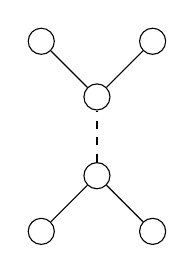
\begin{tikzpicture}
          \node[draw,circle] (1) {};
          \node[draw,circle,below right of=1] (2) {};
          \node[draw,circle,below left of=1] (3) {};

          \node[draw,circle,above of=1] (4) {};
          \node[draw,circle,above right of=4] (5) {};
          \node[draw,circle,above left of=4] (6) {};

          \path[dashed] (1) edge (4);

          \path[-]
          (1) edge (2)
          (1) edge (3)
          (4) edge (5)
          (4) edge (6);
        \end{tikzpicture}
      \end{figure}
  \end{itemize}

\end{frame}


\section{Rückwärtssuche}
\sectionframe{\insertsection}
\begin{frame}{\insertsection}
  \begin{itemize}
    \item<+-> Eingabeparameter \texttt{n}, \texttt{i}, \texttt{upper\_bound}
    \item<+-> entfernt Vergleiche in jedem Schritt
    \item<+-> startet bei Poset $(1, 0, \emptyset)$ % gelöstes Poset an Tafel
    \item<+-> berechnet iterativ alle in $k$ Schritten lösbaren Posets % k Werte Tafel
    \item<+-> terminiert, wenn Poset $(n, i, \emptyset)$ gefunden % leeres Poset Tafel
  \end{itemize}
\end{frame}

\begin{frame}{Vorgängerberechnung}
  \begin{definition}[Vorgänger]
    Poset $Q$ ist Vorgänger von Poset $P$, wenn folgende Bedingungen erfüllt sind:
    \begin{itemize}
      \item<+-> $P$ und $Q$ sind normalisiert % Achtung: eindeutige Normalform
      \item<+-> $Q$ wurde in keiner früheren Ebene gefunden % (otherwise it would be solvable in fewer comparisons)
      \item<+-> durch Hinzufügen eines Vergleich $(i, j)$ in $Q$ resultiert $P$ % Achtung: anschließende Normaliserung
      \item<+-> durch Hinzufügen von $(j, i)$ resultiert ein bereits bekanntes Poset % und anschließende Normalisierung
    \end{itemize}
  \end{definition}
\end{frame}

% nicht weiter, an dieser Stelle Beispiel

\begin{frame}{Beispiel}
  % Idee: interaktiv an Tafel
  % Ebene k enthält alle Posets, die in k Vergleichen gelöst werden können und durch vorherigen Ebene(n) gebildet werden können
  % ganze Pfeile: zeigen auf Poset in Ebene k - 1, das durch Entfernen eines Vergleichs resultiert
  % gestrichelte Pfeile: zeigen auf Poset, das resultiert Umkehrvergleich eingefügt wird (alle Ebenen kleiner k)
  % Rückwärtssuche startet unten bei k = 0, einzigem "gelösten" Poset
  % berechne Ebene k + 1 wie folgt:
  %  - versuche zunächst einen Vergleich zu entfernen
  %  - füge Element mit Vergleichen hinzu, sodass lösbarkeit nicht beeinfluss & entferne anschließend Vergleich
  %  - 

  \begin{figure}[!b]
    \centering
    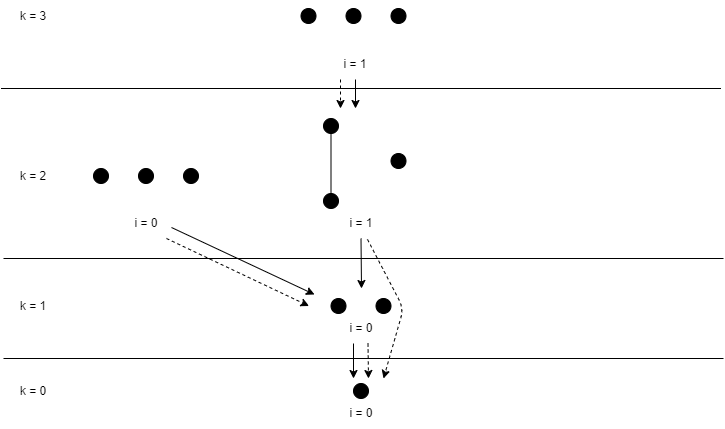
\includegraphics[width=0.9\textwidth,height=0.67\textheight,keepaspectratio]{./figures/backward-searchtree-bound3.png}
    \caption{Suchbaum für $n=4,i=1,\text{upper\_bound}=3$}
    \label{fig:backward-searchtree-bound3}
  \end{figure}
\end{frame}

\begin{frame}{Beispiel}
  \begin{figure}[!b]
    \centering
    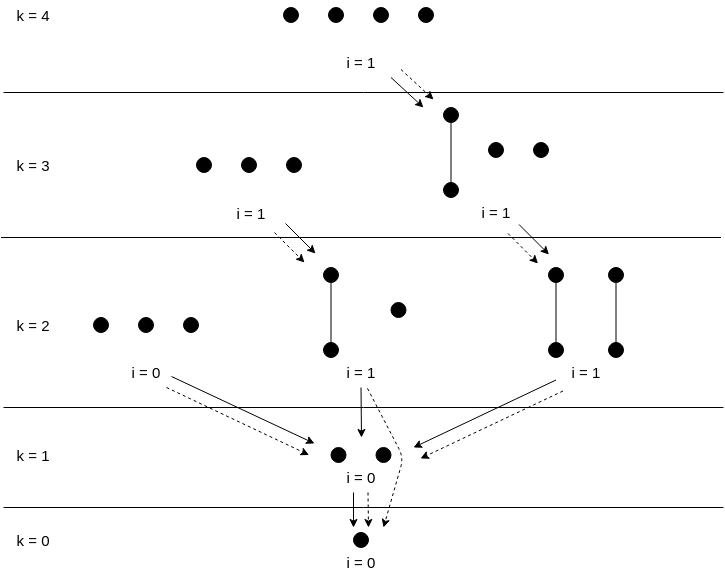
\includegraphics[width=0.9\textwidth,height=0.67\textheight,keepaspectratio]{./figures/backward-searchtree-bound4.png}
    \caption{Suchbaum für $n=4,i=1,\text{upper\_bound}=4$}
    \label{fig:backward-searchtree-bound4}
  \end{figure}
\end{frame}

\begin{frame}{Optimierung}
  \begin{table}[!t]
    \renewcommand{\arraystretch}{1.2}
    \centering
    \begin{tabular}{c|cccc}
      $n$ & \multicolumn{4}{c}{$i$}             \\
          & 0                       & 1 & 2 & 3 \\ \hline
      7   & -                       & - & - & x \\
      6   & -                       & - & x & - \\
      5   & -                       & x & x & - \\
      4   & x                       & x & - & - \\
      3   & x                       & x & - & - \\
      2   & x                       & - & - & - \\
      1   & x                       & - & - & - \\
    \end{tabular}%
    \caption{Mögliche Vorgänger für $n = 7,i = 3$}
  \end{table}
\end{frame}

\begin{frame}{Entfernen von Vergleichen}
  \centering
  \begin{tikzpicture}
  \node[circle,draw=black] (A1) at (0, 0) {};
  \node[circle,draw=black] (A2) at (0, 1) {};
  \node[circle,draw=black] (A3) at (0, 2) {};

  \draw (A1) -- (A2) node {};
  \draw (A2) -- (A3) node {};
  \node (AL) at (0, -0.5) {$i = 1$};
  \node (A) at (0, -1) {(1)};


  \node[circle,draw=black] (B1) at (2.5 + 0, 0) {};
  \node[circle,draw=black] (B2) at (2.5 + 0, 2) {};
  \node[circle,draw=black] (B3) at (2.5 + 1, 1) {};

  \draw (B1) -- (B2) node {};
  \node (BL) at (2.5 + 0.5, -0.5) {$i = 1$};
  \node (B) at (2.5 + 0.5, -1) {(2)};


  \node[circle,draw=black] (C1) at (5 + 1, 2) {};
  \node[circle,draw=black] (C2) at (5 + 0, 0) {};
  \node[circle,draw=black] (C3) at (5 + 2, 0) {};

  \draw (C1) -- (C2) node {};
  \draw (C1) -- (C3) node {};
  \node (CL) at (5 + 1, -0.5) {$i = 1$};
  \node (C) at (5 + 1, -1) {(3)};
\end{tikzpicture}
\end{frame}

\begin{frame}{Kanonifizieren}
  \begin{itemize}
    \item<+-> Kanonifizieren ist unerlässlich
    \item<+-> nauty ist teuer
    \item<+-> z.B. für $n=15,i=7$ wird nur in $0.042\%$ nauty verwendet
  \end{itemize}
\end{frame}

% \begin{frame}{Kanonifizieren}
%   \begin{table}[!t]
%     \renewcommand{\arraystretch}{1.2}
%     \centering
%     \resizebox{\columnwidth}{!}{%
%       \begin{tabular}{c|cccccccc}
%         $n$ & \multicolumn{8}{c}{$i$}                                                          \\
%             & 0                       & 1      & 2     & 3     & 4     & 5     & 6     & 7     \\ \hline
%         13  & 0                       & 30.205 & 6.797 & 1.530 & 0.469 & 0.188 & 0.485 &       \\
%         14  & 0                       & 33.667 & 7.540 & 1.655 & 0.427 & 0.153 & 0.074 &       \\
%         15  & 0                       & 36.390 & 8.173 & 1.683 & 0.460 & 0.133 & 0.066 & 0.042 \\
%       \end{tabular}%
%     }
%   \end{table}
% \end{frame}

\begin{frame}{Multithreading}
  % 1  core : 7h 2m 59s
  % 32 cores:   20m 11s

  \begin{figure}
    \centering
    \resizebox{0.8\textheight}{!}{%
      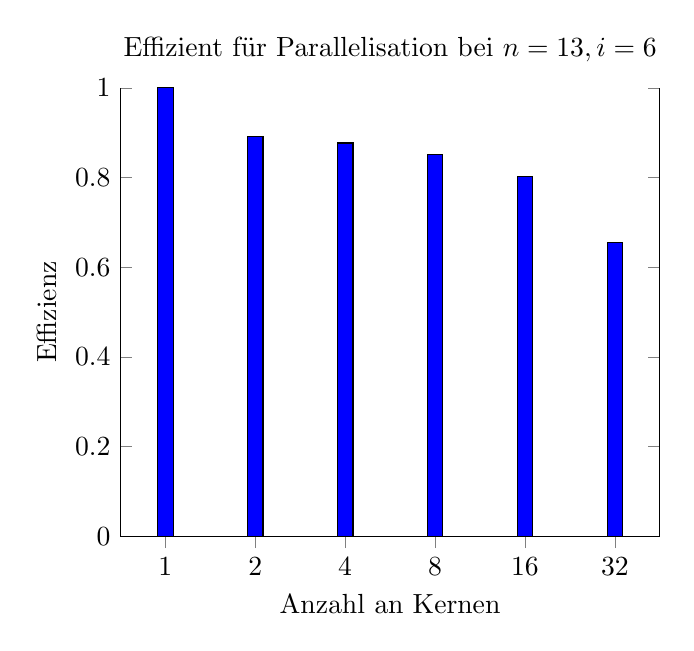
\begin{tikzpicture}
        \begin{axis}[
            ymin=0,
            ymax=1,
            axis x line=bottom,
            enlarge x limits=0.1,
            x axis line style={-},
            ylabel={Effizienz},
            xlabel={Anzahl an Kernen},
            title={Effizient für Parallelisation bei $n = 13, i = 6$},
            ybar, % This makes the plot a bar chart
            bar width=0.2cm, % Adjust bar width
            % nodes near coords, % Display values on top of bars
            xtick=data, % Set x-ticks to data points
            symbolic x coords={1, 2, 4, 8, 16, 32}, % Specify the x-tick labels
          ]
          \addplot[
            ybar,
            fill=blue
          ] coordinates {
              (1, 1.000)
              (2, 0.892)
              (4, 0.877)
              (8, 0.851)
              (16, 0.803)
              (32, 0.655)
            };
        \end{axis}
      \end{tikzpicture}%
    }
  \end{figure}

  $\text{efficiency} = (\text{single-core time}) \div (\text{number of cores} \cdot \text{multi-core time})$ \\
\end{frame}

\begin{frame}{Poset Verteilung}
  \begin{figure}[!b]
    \centering
    \resizebox{0.9\textheight}{!}{%
      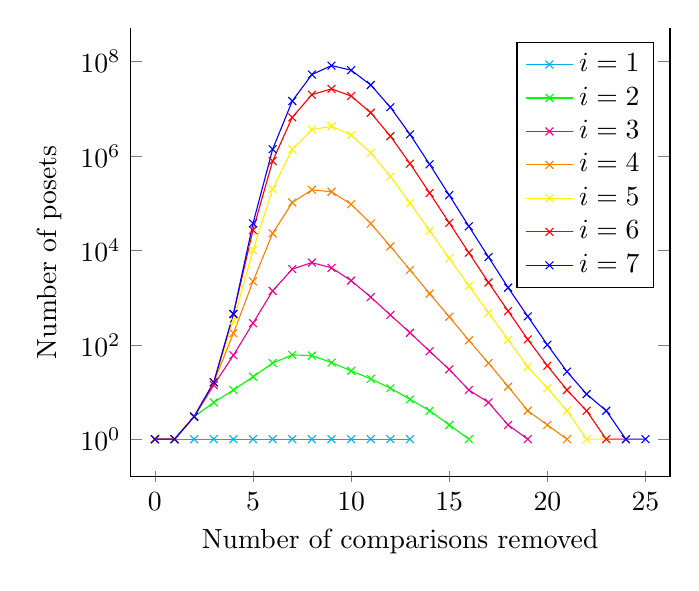
\begin{tikzpicture}
  \begin{axis}[
      ymode=log,
      axis x line = bottom,%x-Achse nur unten
      % x dir=reverse,
      enlarge x limits = .05,%x-Achse erweitern
      x axis line style = {-},%kein Pfeil
      % title = {\dots},
      ylabel={Number of posets},
      xlabel={Number of comparisons removed},
      % only marks,
      cycle list={{mark=x}},
      legend pos=north east,
    ]
    \addlegendentry{$i = 1$}
    \addplot+[cyan] table { %n=14,i=0
        x  y
        0  1
        1  1
        2  1
        3  1
        4  1
        5  1
        6  1
        7  1
        8  1
        9  1
        10 1
        11 1
        12 1
        13 1
      };
    \addlegendentry{$i = 2$}
    \addplot+[green] table { %n=14,i=1
        x y
        0  1
        1  1
        2  3
        3  6
        4  11
        5  21
        6  41
        7  61
        8  59
        9  42
        10 28
        11 19
        12 12
        13 7
        14 4
        15 2
        16 1
      };
    \addlegendentry{$i = 3$}
    \addplot+[magenta] table { %n=14,i=2
        x y
        0  1
        1  1
        2  3
        3  14
        4  60
        5  287
        6  1385
        7  4005
        8  5510
        9  4268
        10 2284
        11 1025
        12 428
        13 180
        14 73
        15 30
        16 11
        17 6
        18 2
        19 1
      };
    \addlegendentry{$i = 4$}
    \addplot+[orange] table { %n=14,i=3
        x y
        0  1
        1  1
        2  3
        3  16
        4  175
        5  2201
        6  22900
        7  103210
        8  191627
        9  174416
        10 94785
        11 37004
        12 12173
        13 3851
        14 1211
        15 392
        16 124
        17 41
        18 13
        19 4
        20 2
        21 1
      };
    \addlegendentry{$i = 5$}
    \addplot+[yellow] table { %n=14,i=4
        x y
        0  1
        1  1
        2  3
        3  16
        4  323
        5  10111
        6  200521
        7  1386176
        8  3607272
        9  4267576
        10 2763862
        11 1162696
        12 367875
        13 100552
        14 26024
        15 6745
        16 1781
        17 474
        18 127
        19 34
        20 12
        21 4
        22 1
        23 1
      };
    \addlegendentry{$i = 6$}
    \addplot+[red] table { %n=14,i=5
        x y
        0  1
        1  1
        2  3
        3  16
        4  446
        5  26921
        6  780123
        7  6588569
        8  19882832
        9  26416869
        10 18631911
        11 8243306
        12 2630332
        13 688904
        14 164372
        15 38334
        16 8918
        17 2084
        18 518
        19 130
        20 36
        21 11
        22 4
        23 1
        24 1
      };
    \addlegendentry{$i = 7$}
    \addplot+[blue] table { % n=14,i=6
        x y
        0  1
        1  1
        2  3
        3  16
        4  452
        5  37236
        6  1389385
        7  14591680
        8  53003482
        9  82198656
        10 65707713
        11 31909980
        12 10770689
        13 2864659
        14 665109
        15 147573
        16 32349
        17 7214
        18 1624
        19 400
        20 100
        21 27
        22 9
        23 4
        24 1
        25 1
      };
  \end{axis}
\end{tikzpicture}
    }
    \caption{Anzahl Posets für $n = 14$ in Abhängigkeit von Anzahl der Vergleiche}
  \end{figure}
\end{frame}


\section{Bidirektionale Suche}
\sectionframe{\insertsection}
\begin{frame}{\insertsection}
  % Idee

  \begin{itemize}
    \item<+-> Idee: Vorwärts- und Rückwärtssuche gleichzeitig starten
    \item<+-> Problem:
      \begin{itemize}
        \item<+-> Cachezugriffe (analog Vorärtssuche)
        \item<+-> Verteilungen der Vergleiche haben ungünstige Massen - siehe [Folie \ref{fig:massen}]
        \item<+-> Rückwärtssuche kann keine Vergleiche ausschließen und die Vorwärtssuche nicht unterstützen
      \end{itemize}
  \end{itemize}
\end{frame}

\begin{frame}{\insertsection}
  \begin{figure}[!b]
    \centering
    \renewcommand{\arraystretch}{0.9}
    \resizebox{0.85\textheight}{!}{%
      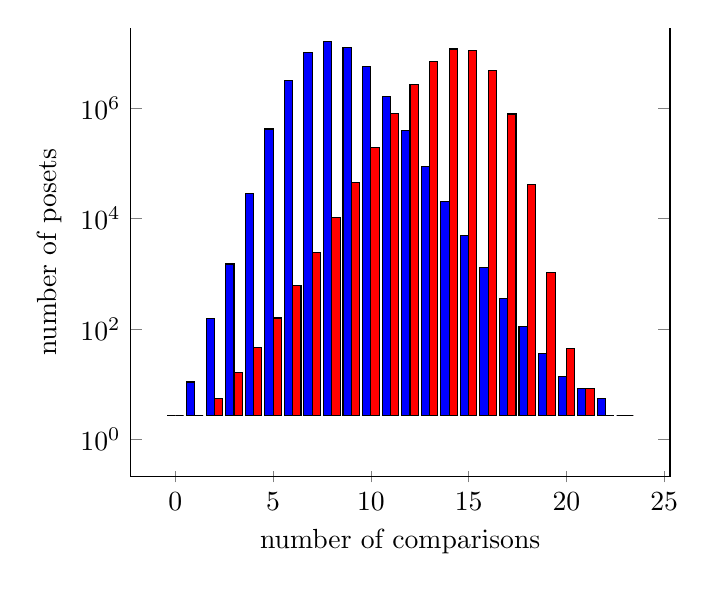
\begin{tikzpicture}
  \begin{axis}[
      ybar,
      ymode=log,
      axis x line = bottom,%x-Achse nur unten
      enlarge x limits = .1,%x-Achse erweitern
      x axis line style = {-},%kein Pfeil
      bar width=3pt,
      ylabel={number of posets},
      xlabel={number of comparisons},
      % legend cell align=left,
      % legend pos=outer north east,
      % legend style={at={(0.5,-0.2)},anchor=north}, % draw=none
    ]
    % \addlegendentry{forward search}
    \addplot[fill=blue,shift={(1pt, 0)}] table {
        x y
        0  1
        1  4
        2  57
        3  552
        4  10397
        5  154828
        6  1166640
        7  3770182
        8  5941732
        9  4726819
        10 2096404
        11 604582
        12 143058
        13 32460
        14 7450
        15 1823
        16 471
        17 132
        18 41
        19 13
        20 5
        21 3
        22 2
        23 1
      };
    % \addlegendentry{backward search}
    \addplot[fill=red,shift={(-1pt, 0)}] table {
        x y
        23 1
        22 1
        21 3
        20 16
        19 381
        18 15227
        17 290138
        16 1750707
        15 4058631
        14 4368185
        13 2592437
        12 1006071
        11 291970
        10 72346
        9  16728
        8  3898
        7  893
        6  227
        5  58
        4  17
        3  6
        2  2
        1  1
        0  1
      };
  \end{axis}
\end{tikzpicture}

Treff: 11
      %\caption{$n = 13$ and $i = 6$}
      % \label{fig:backward_forward_count_13_6}
      \label{fig:massen}
    }
  \end{figure}

  {\color{red} Rot: Rückwärtssuche},
  {\color{blue} Blau: Vorwärtssuche}

  % erkläre, warums net geht
\end{frame}


\section{Ergebnisse}

\begin{frame}{\insertsection}
  \begin{itemize}
    \item<+-> Bestätigung der Vergleiche von Oksanen
    \item<+-> Generierung der Algorithmen für gefundene Anzahl an Vergleiche
    \item<+-> Verifizierung der gefunden Algorithmen
    \item<+-> Verbesserung der Schranke von Oksanen (e.g. $n=15$, $i=4$)
    \item<+-> Weiterer untere Schranken für $n=15$ - siehe Tabelle [Folie \ref{tab:results}]
  \end{itemize}
  % hier kommt fehler von oksanen hin (falsche Heuristik,, führt zu falschem wert)

  % hier kommt faslche these von gasarch

  % hier kommt hin: Lemma 1 ist auch ein neues Ergebniss, dass weder Oksanen noch Gasarch rausgefunden haben (zumindest nach meinem Wissen; Julius)
\end{frame}

\begin{frame}{\insertsection}
  \begin{table}[!t]
    \label{tab:results}
    \renewcommand{\arraystretch}{0.9}
    \centering
    \resizebox{0.85\textheight}{!}{%
      \begin{tabular}{c|cccccccc}
        \backslashbox{$n$}{$i$} & 0  & 1  & 2  & 3  & 4                    & 5           & 6           & 7           \\ \hline
        1                       & 0                                                                                  \\
        2                       & 1                                                                                  \\
        3                       & 2  & 3                                                                             \\
        4                       & 3  & 4                                                                             \\
        5                       & 4  & 6  & 6                                                                        \\
        6                       & 5  & 7  & 8                                                                        \\
        7                       & 6  & 8  & 10 & 10                                                                  \\
        8                       & 7  & 9  & 11 & 12                                                                  \\
        9                       & 8  & 11 & 12 & 14 & 14                                                             \\
        10                      & 9  & 12 & 14 & 15 & 16                                                             \\
        11                      & 10 & 13 & 15 & 17 & 18                   & 18                                      \\
        12                      & 11 & 14 & 17 & 18 & 19                   & 20                                      \\
        13                      & 12 & 15 & 18 & 20 & 21                   & 22          & 23                        \\
        14                      & 13 & 16 & 19 & 21 & 23                   & 24          & \textbf{25}               \\
        15                      & 14 & 17 & 20 & 23 & \textbf{\textit{24}} & \textbf{26} & \textbf{26} & \textbf{27} \\
      \end{tabular}%
    }
  \end{table}
\end{frame}

\begin{frame}
  \begin{itemize}
    \item Widerlegen der Behauptung von Gasarch
          \begin{itemize}
            \item Es existiert ein optimaler Algorithmus der zuerst alle Elemente paarweise vergleicht.
            \item Gegenbeispiel: Für $n = 12$, $i = 4$, ergibt die Behauptung eine Grenze von 20
                  Vergleichen, gefunden wurde aber ein Algorithmus mit 19 Vergleichen.
          \end{itemize}
  \end{itemize}
\end{frame}

\begin{frame}

  \begin{table}[!t]
    \label{tab:times}
    \renewcommand{\arraystretch}{1.0}
    \centering
    \resizebox{1.0\textheight}{!}{%
      \begin{tabular}{c|c|l|l|l}
        $n$ & $i$ & \textbf{Forward Search} & \textbf{Backward Search} & \textbf{Oksanen} \\
        \hline
        14  & 0   & 0.0s                    & 0.0s                     & 0.0s             \\
        14  & 1   & 0.0s                    & 1.5s                     & 0.0s             \\
        14  & 2   & 1.4s                    & 5.9s                     & 0.6s             \\
        14  & 3   & 35.9s                   & 46.9s                    & 1m 47s           \\
        14  & 4   & 17m 27s                 & 15m 33s                  & 6h 29m           \\
        14  & 5   & 2h 40m                  & 1h 40m                   & 4d 10h           \\
        14  & 6   & 14h 40m                 & 6h 27m                   & >5d              \\
        \hline
        15  & 0   & 0.0s                    & 0.0s                     & 0.0s             \\
        15  & 1   & 0.1s                    & 4.0s                     & 0.0s             \\
        15  & 2   & 2.8s                    & 25.9s                    & 1.4s             \\
        15  & 3   & 2m 24s                  & 13m 11s                  & 27m 17s          \\
        15  & 4   & 1h 12m                  & 45m 52s                  & 1d 5h 40m        \\
        15  & 5   & 1d 8h 37m               & 19h 30m                  & >5d              \\
        15  & 6   & 4d 23h 37m              & 1d 5h 43m                & >5d              \\
        15  & 7   & 14d 1h 51m              & 3d 8h 9m                 & >5d              \\
      \end{tabular}
    }
  \end{table}
\end{frame}

\thanksframe

% \begin{frame}{Quellen}
%   \nocite{*}
%   \printbibliography
% \end{frame}